
%\documentclass[conference]{IEEEtran}
\documentclass{sig-alternate}

\clubpenalty=10000
\widowpenalty = 10000

\newcommand{\todo}[1]{\textcolor{cyan}{\textbf{[#1]}}}
\newcommand{\sam}[1]{\textcolor{red}{{\it [Sam says: #1]}}}
\newcommand{\dan}[1]{\textcolor{blue}{{\it [Dan says: #1]}}}

% --- Author Metadata here ---
\conferenceinfo{SAC'16,}{April 4-8, 2016, Pisa, Italy.}
\CopyrightYear{2016} % Allows default copyright year (2002) to be over-ridden - IF NEED BE.
\crdata{978-1-4503-3739-7/16/04...\$15.00.\\
http://dx.doi.org/xx.xxxx/xxxxxxx.xxxxxxx
}  % Allows default copyright data (X-XXXXX-XX-X/XX/XX) to be over-ridden.
% --- End of Author Metadata ---



\usepackage{cite}
\usepackage{listings}
%\usepackage{booktabs}
\usepackage{color}
\usepackage{balance} % Helps to balance out text on last page
\usepackage{url}
\usepackage{times} % Used for formatting formatting url footnotes
\urlstyle{same} % Used for formatting formatting url footnotes

\usepackage{graphicx} % Including images


%%% Not sure if these can be removed
\usepackage{tikz}
\usetikzlibrary{shapes, arrows, positioning}
\usetikzlibrary{patterns}


%%% Everything below is used for the confusion matrix
%%%% This needs to be cleaned up a bit
\usepackage{array}
\usepackage{multirow}


\usepackage{pgfplots} % needed for bar chart


\pdfpagewidth=8.5in
\pdfpageheight=11in


\newif\ifisnopii
%\isnopiitrue % change to true/false to remove personally identifiable information (pii)
\isnopiifalse % change to true/false to remove personally identifiable information (pii)


%%% For adding line breaks in cells
\newcommand{\specialcell}[2][c]{%
  \begin{tabular}[#1]{@{}l@{}}#2\end{tabular}}



\begin{document}

% Making Bug Fixing Easier in Android Apps
% Fixing Bugs Sooner: An Analysis of Android Defects and their Repair Process


\title{Evaluating Effectiveness of Static Analysis Testing Tools On Android Applications}

\numberofauthors{1}
\ifisnopii % turn on/off pii
\author{
%
% 1st. author\
\alignauthor
%Daniel~E.~Krutz, Patrick McAfee, \&~Samuel~A.~Malachowsky\\ 	
XXXXXX \\
	\affaddr{Software Engineering Department}\\
       \affaddr{Rochester Institute of Technology}\\
       \affaddr{1 Lomb Memorial Drive}\\
       \affaddr{Rochester, NY, USA} \\
       \email{\{dxkvse, XXXX\}@rit.edu}
       \alignauthor
} % Must not be a space above this

\else % turn on/off pii
\author{
%
% 1st. author
\alignauthor
xxxxxxxxxxxxxxx\\ 	
	\affaddr{xxxxxxxxx}\\
       \affaddr{xxxxxxxxx}\\
       \affaddr{xxxxxxxxx}\\
       \affaddr{xxxxxxxxx, xx, xxx} \\
       \email{xxxxxx@xxxxx.xxx}
       \alignauthor
} % Must not be a space above this
\fi % end turn on/off pii


\maketitle

\begin{abstract}
Mobile applications (apps) have taken the computing world by storm. On the Android platform alone, there are over a million apps available for download on over one billion Android devices. Android development can be very lucrative, but is also extremely competitive due to the number of options that users have. Users will often choose alternative apps over ones which are delivered late or are buggy. Developers are under an immense amount of pressure to create apps quickly, and make them as high quality as possible. Static analysis testing tools are often relied upon to automatically perform a brunt of the testing to quickly and cheaply discover possible errors in the app. Unfortunately, all static analysis tools are not created equal.

In the following paper, we investigate the effectiveness of three leading static analysis testing tools for Android: FindBugs, PMD and Android Lint. We first created a defect oracle of fifty unique errors from eight defect categories and then ran the tools against this oracle comparing the results of our examined tools in terms of precision, recall, and F-measure. Our primary contributions of this work are an unbiased analysis of these three leading testing tools, along with a publicly accessible defect oracle which may be used for future evaluations and research.

While none of the three tools led in all evaluated categories, FindBugs performed at the most consistently high level and led in the categories of Recall and F-measure.

%\todo{clean up page spacing and formatting}
% \vspace{30mm}

\end{abstract}

%% Categories taken from: http://www.jucs.org/ujs/jucs/links/Articles%20by%20Category/D.?mode=bc

%% Not sure if this should be added back in?
%\category{D.2.4}{Software Engineering} Software/Program Verification
\category{D.2.5}{Software Engineering} Testing and Debugging


\keywords{Android, Testing, Static Analysis}


\section{Introduction}
Mobile apps have changed the way that we live and work allowing for an unprecedented level of power at almost any time in any location. There are currently over one million Android apps~\cite{AppBrain_URL} on over one billion devices~\cite{jenniferscott2014} which give developers a wide range of customers, but also give customers a diverse range of options. For many users, a deciding factor for the app they will choose is its quality, which they may witness firsthand or may read from reviews of the app~\cite{khalidexamining}.

Developers are under an immense amount of pressure to deliver apps and their updates in a prompt, cost effective and high quality manner. Static analysis tools are routinely used to quickly, and automatically test apps for a variety of problems including defects~\cite{johnson2013don} and security vulnerabilities~\cite{Ware:2008:SJC:1394504.1394506, song2015finding}. Static analysis tools evaluate a system and its components without actually executing the software~\cite{159342}.

Android developers often use static analysis tools to assist with defect detection. Unfortunately, not all static analysis tools are created equally. \emph{The goal of our research is to evaluate static analysis tools that are used for testing Android applications.} We evaluated three leading Android static analysis testing tools: FindBugs~\cite{FindBugs_URL}, PMD~\cite{Rutar:2004:CBF:1032654.1033833}, and Android Lint~\cite{AndroidLint_URL} assessing them in a variety of areas including precision, recall and F-measure. In our comparison of the tools, we sought to answer the following research questions:\\


%Mobile applications, more commonly known as ?apps?, have gained immense popularity since the beginning of the new millennium. They have become an important part of life in the twenty first century and are used to accomplish critical daily tasks. As of February 2015, the Google Play Store surpassed 1.4 million apps for digital download and installation [5]\todo{fix}. Digital channels, such as the Google Play Store, can be accessed directly from a mobile device connected to the internet, giving users the ability to continuously install, update, and delete their apps. Due to this, users have been conditioned with a low tolerance for software defects in a released app because of the ease with which they can download and install a functionally similar one of higher quality. Producing high quality software releases, therefore, becomes essential when trying to compete in the extremely volatile marketplace. This means that mobile application projects need to have the ability to identify defects quickly, continuously, and effectively.

% Static analysis tools provide quick feedback on the current quality of the software under test. These tools, generally, are available as plugins for integrated development environments (IDEs) and can be easily installed and run at any point in the software lifecycle. Mobile application project teams would greatly benefit from using static analysis tools to quickly identify potential software defects and work towards implementing changes to mitigate the risk of releasing a poor quality version of the application to the unforgiving marketplace.

%In this study we investigate three static analysis tools available for mobile applications developed for the Android operating system: FindBugs\footnote{\url{http://findbugs.sourceforge.net}}, PMD~\cite{Rutar:2004:CBF:1032654.1033833}, and Android Lint\footnote{\url{http://developer.android.com/tools/help/lint.html}}. We compare these three static analysis tools by running them on open source Android applications. Using the defects gathered from these apps, we are able to compare the effectiveness of the tools and make recommendations to the Android mobile application development and research communities. These recommendations can be used by product teams to instill confidence in app releases and inspire future research in this area.

%

%% Check format of how other papers do this


%\noindent
\textbf{RQ1:}~\emph{What categories of defects are found by static analysis tools?}\\
We categorized defects into eight different groups including `compatibility', `concurrency', `correctness', `maintainability', `performance', `reliability', `security', and `usability.' We found that PMD discovered defects in 6/8 of the groups, while FindBugs identified defects in 5/8 and Android Lint only found defects in 2/8 groups. \\



%\todo{merge this with RQ1?}
%\noindent
%\textbf{RQ2:}~\emph{What are the similarities and differences between the available static analysis tools?}\\
%We next analyzed the discovered defects from each static analysis tool in an in-depth manner to better understand what groups and types of defects each tool was able to discover in comparison with one another.
%FindBugs was able to detect the most high priority potential defects while PMD found the most performance and reliability defects. Android Lint was strong in detecting defects related to Android specific faults, as expected according to the documentation, but was extremely weak in detecting defects in the common Java code.


% FindBugs was able to detect the most high priority potential defects, as well as identifying the most potential defects in the following categories: concurrency, correctness, and security. PMD found the most performance and reliability defects and was the only tool to find maintainability and usability defects. Android Lint was strong in detecting defects related to Android specific faults, as expected according to the documentation, but was extremely weak in detecting defects in the common Java code.


%\noindent
\textbf{RQ2:}~\emph{Which static analysis tool is the most effective at finding defects?}\\
We evaluated each tool against the known bugs in our oracle in terms of precision, accuracy and F-measure. While no tool led in all three areas, FindBugs discovered defects at the most consistently high level in each category. \\

%To answer the above research questions, we examined multiple static analysis tools in parallel on select Android mobile applications to perform our evaluation. Our methodology included the following steps: choose three static analysis tools, create a defect oracle containing various defect patterns, run each tool on three different Android applications, match discovered defects with the defect patterns from the oracle, and calculate statistics to determine the effectiveness of each tool.

%The remainder of this paper is organized as follows: Section~\ref{sec: ourexperiences} describes our experi\dan{make sure this is up to date}

The remainder of this paper is organized as follows: Section~\ref{sec:related} discusses previous work with static analysis tools. Section~\ref{sec:Methodology} provides the methodology we used to conduct our analysis. The results of our analysis are provided and discussed in Section~\ref{sec:results}, while Section~\ref{sec:publicdataset} provides information about our public data set which may be accessed and used by other researchers. Section~\ref{sec:limitations} discusses limitations of our study and future work to be conducted while Section~\ref{sec:conclusion} provides a conclusion of our study.

\newpage
\section{Related Work}
\label{sec:related}


The importance of static analysis tools have been demonstrated in innumerable ways with research being dedicated to improving their performance while reducing their false positives~\cite{joshi2014reducing}. Static analysis tools have been developed for a variety of purposes for a range of programming languages and platforms including defect detection~\cite{johnson2013don} and security analysis~\cite{Ware:2008:SJC:1394504.1394506, song2015finding, Feng:2014:ASD:2635868.2635869, Schmeelk:2015:AMS:2746266.2746271}. There are also a wide range of testing tools developed for Android apps including GUI testing~\cite{Hu:2011:AGT:1982595.1982612}, tools which relied upon symbolic analysis~\cite{Mirzaei:2012:TAA:2382756.2382798}, and those that found bugs using pattern analysis~\cite{6924298}. There are even static analysis testing tools that search for energy leaks in apps~\cite{Zhang:2012:AAD:2380445.2380503,}, and examine for cache performance~\cite{banerjee2013static} and those that measure defect density~\cite{Nagappan:2005:SAT:1062455.1062558}.

Studies have compared the effectiveness of various static analysis tools. Rutar et al.~\cite{Rutar:2004:CBF:1032654.1033833} evaluated several leading static analysis tools on Java applications. They found that no single static analysis tool should ever be deemed to be perfect and made the argument for the concurrent use of several tools to ensure maximum testing coverage. While this work was profound, it did not evaluate the tools against one another, or create an oracle to measure the precision, recall or F-measure of the tools.

Research has also examined how static analysis testing tools are used in the real world. Ayewah et al.\cite{4602670} reported on their experiences running FindBugs against Sun's JDK and at Google where it was integrated into their standard development process. Some of their reported findings included the lack of perceived value that many developers had in running static analysis testing tools, and that developers pay the most attention to high priority issues. They also found that users are typically less likely to repair defects found in older code.


%%%% Not sure how much of this is relevant and how much fluff I am just putting in. I will leave out for now.
%%Bessey et al.\cite{Bessey:2010:FBL:1646353.1646374} also studied the use of static anlaysis tools in the real world and found that surprisingly high number of developers did not care about


Thung et al.\cite{Thung:2012:EWD:2351676.2351685} examined the extent that field defects were discovered using several leading static analysis tools including FindBugs, PMD, and JLint. They found that while many field defects could be identified by these tools, a significant portion of issues were not identified. This work also characterized many of the missed defects. %Unfortunately, there does not appear to have been any work in this area which used the actual Android source code as part of its analysis.

Previous research has demonstrated the importance of having high quality apps and their direct impact on user ratings. Khalid et al.\cite{7006337} examined the relationship of code quality (using FindBugs) and the app's user rating. They found that ``Bad Practice'', ``Internationalization'' and ``Performance'' error categories were much more common in lower rated compared to high-rated apps. The work also found a direct correlation between these defects and complaints in the app's reviews. They determined that app developers could raise their use rating by resolving these specific types of defects using static analysis tools.

%%% Not sure how this applies to this paper
%Harman et al.~\cite{6224306} examined 32,108 non-zero priced apps and found a strong correlation between customer rating and the rank of app downloads and that there was no correlation between app price and rating. This demonstrates the importance of user ratings and perception on the popularity of an app.



%% Many studies have evaluated the use of Static analysis tools in various areas
%	- Using FindBugs On Production Software



%\todo{probably add more to related work. This should help to beef up the paper}



\section{Methodology}
\label{sec:Methodology}


The goal of our research is to evaluate the quality of three leading static analysis tools for Android. Effective static analysis defect detectors are important so developers may be sure that their tools are discovering a significant portion of the actual defects in the app, but are not returning a high level of false positives. In order to evaluate the static analysis tools, we first created a defect oracle containing various defect patterns, ran each tool on three different Android applications, matched discovered defects with the defect patterns from the oracle, and then calculated statistics to determine the effectiveness of each tool. In the following sections, we will describe the tools, our defect oracle, and how the tools were ran. The purpose is to not only provide a background of how we attained our results, but to allow future researchers to re-run our analysis should they choose to do so.

\subsection{Selected Tools}
We selected three leading static analysis tools for our comparison: FindBugs, PMD, and Android Lint. We chose these tools based upon their popularity and their use in previous work~\cite{7006337, Thung:2012:EWD:2351676.2351685}. The tools are briefly described below: \\


\noindent
\textbf{FindBugs}

A popular open source static analysis tool that examines files for detects using approximately 300 pre-defined bug patterns. Each FindBugs defect pattern is categorized based on correctness, bad practice, performance, and internationalization. FindBugs also rates the reported bugs based on its confidence and rank level. The confidence is based how certain - low, medium, or high - the tool is that the identified defect will result in a failure. The rank level - of ``concern'', ``troubling'', ``scary'', or ``scariest'' - is how much of a problem the identified defect is likely to be. For example, an unused variable may be rated as troubling, while a memory leak may be rated as scary. In our analysis, we used FindBugs in the Android Studio IDE.\\


\noindent
\textbf{PMD}

This tool detects potential defects in software written in Java. When performing the code analysis, the tool compares syntax patterns against predefined PMD rulesets. These rulesets define various categories of bad practices and potential bugs. Each ruleset is classified as one of the following categories: efficiency, maintainability, reliability, and usability. Each identified defect is rated based on the severity - ``minor'', ``major'', ``critical'', or ``blocker''. PMD reports all detected warnings and unlike FindBugs, does not rate them based on confidence. This leads to a large number of warnings that may contain false positives.\\
%% Make sure to talk about how we used the android settings


\noindent
\textbf{Android Lint}

A static analysis tool that is dedicated to Android development. This tool is provided by the Android SDK and is the default inspection tool used in the Android Studio IDE. In addition to Java code analysis, the tool also analyzes compatibility of the code with the various versions of the Android API. The tool reports issues with the structural quality of the source code and each issue is reported with a message and a severity level used for prioritization. Android Lint may be ran from the command line or from Android studio. In our analysis, we ran Android Lint from the command line.\\



\subsection{Defect Oracle}
%% Unbaised since we were not trying to demonstrate the power of any single tool

An important goal of our work was to create an unbiased, high quality defect oracle that could also be used for future tool evaluations. The defect oracle is a repository of defects used to analyze the effectiveness of the three static analysis tools. Each tool contains a set of defect patterns that are used during code inspections to identify defects and each of these defect patterns are unique to the tool itself and cannot be directly compared to other tools. In order to provide a common set of potential defects the following procedure was performed:

Step 1: Identify the common defect patterns for each tool:
Since there are hundreds of possible defect patterns among the tools, we limited our research to only use high-priority patterns. This resulted in a total of fifty nine defect patterns compiled from all three static analysis tools. We analyzed each of the fifty nine pattern descriptions and determined which patterns were duplicates. From this analysis, we were able to identify fifty unique defect patterns, which were added to the defect oracle.

Step 2: Create a unique defect identifier that maps to each tool's defect pattern:
Each defect pattern was assigned a unique defect identifier. If the defect pattern was determined to be a duplicate between multiple tools, we mapped the tool's defect pattern description to the unique defect identifier in the defect oracle. This step was essential for tracking defects discovered by multiple tools with different defect naming conventions.

Step 3: Analyze, describe, and categorize each defect:
We created a common defect description for each defect identifier and sorted them into the following categories: compatibility, concurrency, correctness, maintainability, performance, reliability, security, and usability. %Table~\ref{Table:defectdescriptionmapping} shows the mapping of the oracle defect descriptions to each tools defect descriptions.\todo{Is the table needed?}


%\begin{table*}[h]
%\begin{center}
%\caption{Defect Description Mapping}
%\label{Table:defectdescriptionmapping}
%  \begin{tabular}{ | l | l | l | c | c | c | c | c | c | c | } \hline
%
%     \bfseries DefectID  & \bfseries Bug Category & \bfseries Our Bug Description & \bfseries Priority & \bfseries Mapped PMD Bug Description  \\  \hline
%
%	1 & Compatibility & \specialcell{ Right-to-left text compatibility issue from\\ API 17 to specified API 14} & 1 & \todo{why none?} \\ \hline	
%	2 & Maintainability & Empty Catch Block & 5 & Avoid empty catch blocks  \\ \hline
%	
%	3 & Maintainability & Empty if statement & 5  & Avoid empty if statements \\ \hline	
%	4 & Reliability & Switch statement missing break & 3  & A switch statement does not contain a break \\ \hline
%
%  \end{tabular}
%  \end{center}
%\end{table*}


% \noindent
Step 4: Determine if the item is actually a defect.: We manually examined each of the potential defects in the oracle and ranked them 1-5 based on the likelihood of resulting in a failure; 1 most likely a defect, 5 least likely a defect. Table~\ref{Table:rankeddefects} shows an example subset of the ranked defects in the oracle.  The `Reliability' defect  is ranked low (5) since it most likely wouldn't cause an issue, but it still may be a security concern. The `Correctness' defect has a high (1) priority due to our certainty that the item is a real defect and would very likely lead to a problem if encountered by the application. This defect describes a guaranteed null pointer de-reference which would generate a null pointer exception when the code is executed. We ranked defects by first ranking them independently, and then discussed any differences until an agreement could be made. While we acknowledge that this is an imperfect process, we feel that it is more than sufficient for our oracle and that virtually any ranking system, whether done by tool or manual process, is going to carry at least some subjectivity.

\begin{table}[h!]
%% Former:  F3-2
%% \specialcell{ Right-to-left text compatibility issue\\ from API 17 to specified API 14}
\begin{center}
\caption{Example Ranked Defects}
\label{Table:rankeddefects}
  \begin{tabular}{ | l | c | c | } \hline

     \bfseries Bug Category & \bfseries Our Bug Description & \bfseries Priority  \\  \hline

          Reliability & Incorrect switch statement & 5  \\ \hline
          Performance & Calls garbage collection explicitly & 3  \\ \hline
          Concurrency & Unsynchronized lazy initialization & 3  \\ \hline
          Correctness & Null pointer de-reference & 1  \\ \hline

  \end{tabular}
  \end{center}
\end{table}

We have made the oracle available for public use on our project website: \ifisnopii \url{http://darwin.rit.edu/caa/} \else \url{http://hiddenToKeepAnonymous. } \fi.


\subsection{Running the Tools}
We utilized an open source software online catalog called F-Droid\footnote{\url{http://f-droid.org/}} to clone the git repositories of three popular mobile applications: aCal, android-chess, and WordPress. These three applications were chosen because they come from three different domains, greatly vary in size, and were easily imported into the Android Studio IDE.

Each of the three examined tools have different settings which may be altered depending on the desired precision and recall for each tool. In each case, we altered the default settings to create the best precision and recall for each tool. These tool settings are available on our project website.

We next ran each tool on all three applications and extracted the discovered defects upon completion. Each discovered defect was then mapped to the unique defect identifier in the oracle. Table~\ref{Table:tooldescriptionmapping} shows a portion of the mapping of each tool's discovered defects to the defects in the oracle. We will next describe any customized settings made to the tools.\\


\noindent
\textbf{FindBugs}

This popular tool checks for potential defects by using different bug patterns to analyze Java bytecode. Similar to the study conducted by  Khalid et al.\cite{7006337}, we ran FindBugs using its recommended settings which discovers defects that are ``high'' and ``medium'' priority. We ignored ``low'' priority warnings since they contain a significant amount of false positives and is not recommended for analysis~\cite{FindBugs_URL}. Since we were examining duplicated binary of the original code, we ignored all style and naming convention warnings.\\



%In our study, we did not run FindBugs with the default settings. Instead, we tried to maximize the number of potential defects detected by enabling extensions turned off to increase default tool efficiency. Since we were concerned with effectiveness, rather than efficiency, we were willing to accept the tradeoff of longer runtime for a more thorough bytecode analysis. Table~\ref{Table:findbugsettings}  compares the FindBugs default settings to the settings used in this study.\dan{Use findBugs settings from Mei's 10,000 paper}\\

% Examining the Relationship between FindBugs Warnings and End User Ratings: A Case Study On 10,000 Android Apps




\noindent
\textbf{PMD}

This tool looks for potential defects by using different bug patterns to analyzing Java source code. When using PMD, we enabled any detectors turned off by default.\\

\noindent
\textbf{Android Lint}

The third tool is a dedicated Android development static analysis tool and is provided to developers as the default static analysis tool packaged with the Android Studio IDE. Like PMD, Android Lint is not as customizable as FindBugs and only allowed us to enable detectors turned off by default.

%\subsection{Static Analysis Tools}

%% Make sure I copied everything over
%\todo{Is this section missing from the word document.}

\section{Results}
\label{sec:results}

After running the examined tools against our created oracle, we were able to answer our research questions.

\noindent
\emph{RQ1: What categories of defects are found by static analysis tools?}\\
 After running each tool, the reported defects were analyzed and sorted. In total, fifty unique defects were classified into eight categories: compatibility, concurrency, correctness, maintainability, performance, reliability, security, and usability. Table~\ref{Table:defectsbycategory} shows the categorized breakdown of each tool's results.



%\begin{table}[h]
%\begin{center}
%\caption{Identified Defects by Category}
%\label{Table:defectsbycategory}
%  \begin{tabular}{ | l | l | l | l | c | c | c | c | } \hline
%
%     \bfseries  & \bfseries FindBugs & \bfseries PMD & \bfseries Android Lint & \bfseries Total \\  \hline
%
%	Compatibility & 0 & 0 & 7 & 7  \\ \hline
%	Concurrency & 5 & 0 & 0 & 5  \\ \hline
%	Correctness & 9 & 2 & 0 & 11  \\ \hline
%	Maintainability & 0 & 3 & 0 & 3  \\ \hline
%	Performance & 5 & 2 & 2 & 9  \\ \hline
%	Reliability & 1 & 3 & 0 & 4 \\ \hline
%	Security & 8 & 2 & 0 & 10  \\ \hline
%	Usability & 0 & 1 & 0 & 1  \\ \hline
%	\textbf{Total} & \textbf{28} & \textbf{13} & \textbf{9} & \textbf{50}  \\ \hline	
%	
%  \end{tabular}
%  \end{center}
%\end{table}
%%% Make sure all the numbers add up


\begin{table}[h]
\begin{center}
\caption{Identified Defects by Category}
\label{Table:defectsbycategory}
  \begin{tabular}{ | l | c | c | c | c | c |  } \hline

     \bfseries  & \bfseries FindBugs & \bfseries PMD & \bfseries Android Lint \\  \hline

	Compatibility & 0 & 0 & 7   \\ \hline
	Concurrency & 5 & 0 & 0   \\ \hline
	Correctness & 9 & 2 & 0   \\ \hline
	Maintainability & 0 & 3 & 0   \\ \hline
	Performance & 5 & 2 & 2   \\ \hline
	Reliability & 1 & 3 & 0  \\ \hline
	Security & 8 & 2 & 0   \\ \hline
	Usability & 0 & 1 & 0   \\ \hline
	\textbf{Total} & \textbf{28} & \textbf{13} & \textbf{9}  \\ \hline	
	
  \end{tabular}
  \end{center}
\end{table}
%% Make sure all the numbers add up

\begin{table*}[ht]
\begin{center}
\caption{Tool Description Mapping}
\label{Table:tooldescriptionmapping}
  \begin{tabular}{ | l | l | l | c | c | c | c | c | c | } \hline

     \bfseries DefectID  & \bfseries Bug Category & \bfseries Bug Description & \bfseries Priority & \bfseries Tool Priority & \bfseries App(s) & \bfseries PMD & \bfseries FB & \bfseries AL \\  \hline
    %AndroRisk & 56.95 & X \\ \hline

  1 & Compatibility & \specialcell{ Right-to-left text compatibility issue\\ from API 17 to specified API 14}& 1 & Error & WP &  &  & x \\ \hline
  2 & Maintainability & Empty catch block & 5 & Critical & WP, aCHess & x &  &  \\ \hline
  3 & Maintainability & Empty if statement & 5 & Critical & WP, aChess, aCal & x &  &  \\ \hline
  4 & Reliability & Switch statement missing break & 3 & Critical & WP, aChess &  x &  &  \\ \hline
  5 & Security & \specialcell{ Reference to array stored, \\instead of using deep copy} & 2 & Critical & WP, aCal & x & x &  \\ \hline

  \end{tabular}
  \end{center}
\end{table*}



We found that while no tool identified defects in all 8 categories, PMD found defects in 6/8 categories while FindBugs identified defects in 5/8, with Android Lint finding only 2/8. However, FindBugs did discover the most defects with 28 compared to only 13 for PMD and 9 for Android Lint. Based on these results, we can conclude that FindBugs and PMD are both capable of discovering defects in essentially the same number of categories.\\

%\noindent
%\emph{RQ2: What are the similarities and differences between the available static analysis tools?}\\
%The second research question we investigated was comparing the available static analysis tools chosen for this study. \\

%Section 3.1 describes each of the static analysis tools chosen in this study according to their documentation and previous work. Once our first research question was answered, we were able to analyze the similarities and differences between the tools based on the defects collected from each mobile application.

\noindent
\textbf{FindBugs}

FindBugs was able to detect the most high priority potential defects and find the most potential defects in the following categories: concurrency, correctness, and security. Since FindBugs analyzes the compiled Java bytecode, it may not have the ability to detect potential maintainability and usability defects. This is because these categories might require knowledge about how the Java source code is actually written, which is not accessible to FindBugs.\\ %Finally, the FindBugs plugin for Android was unable to detect the compatibility issues found with Android Lint.

\noindent
\textbf{PMD}

PMD found the most performance and reliability potential defects and was the only tool to find potential maintainability and usability defects. Another interesting observation about PMD was that it found more matches to the defect patterns than both FindBugs and Android Lint in all three apps tested; however, the overwhelming majority were not classified as high priority and were deemed out-of-scope for this study. We suspect this is due to PMD analyzing the actual Java source code as written and is reporting potential defects related to coding style.\\

\noindent
\textbf{Android Lint}

Android Lint showed strength in detecting potential defects related to Android specific faults, as expected according to the documentation, but was extremely weak in detecting potential defects in the common Java code. 78\% of the detected defects were specific to compatibility with previous versions of the Android API, while the remaining 22\% were related to garbage collection of allocated memory. Although garbage collection is common to all Java applications and is not specific to Android development, one could argue that development for a mobile environment should be highly concerned with resource usage.\\

We next addressed our second research question:
\emph{RQ2: Which static analysis tool is the most effective at finding defects?}
We sought to determine if a single static analysis tool was the most effective at finding defects using the metrics of precision, recall and accuracy.

\begin{enumerate}
   \setlength{\itemsep}{0pt} %Cut down on spacing for the different items in the list
   \setlength{\parskip}{0pt} %Cut down on spacing for the different items in the list
   \setlength{\parsep}{0pt}  %Cut down on spacing for the different items in the list

  \item~\textbf{Precision:} Ratio of the clone pair which a tool reports that are true clones, not false positives. % Relates the number of files predicted~\emph{and} observed as defect prone to the number of files predicted as defect prone. It is calculated as $\frac{a}{a+b}$.

 \item~\textbf{Recall:} Ratio of the clone pairs in a system that a tool is able to detect. %Relates the number of files predicted~\emph{and} observed as defect prone to the number of files that actually had defects. It is calculated as $\frac{a}{a+c}$.

  \item~\textbf{F-measure:} Considers precision~\emph{and} recall to measure the accuracy of a system. It is calculated as $2\times(\frac{precision\times recall}{precision+recall})$. F-measure is often referred as F1 or F-score.

%%% Don't think this is used in the paper
 %\item~\textbf{Accuracy:} Percentage of elements classified correctly. %It is calculated as $\frac{a+d}{a+b+c+d}$.

\end{enumerate}


%% Not sure if this confusion matrix adds much value
%\begin{table}[t]
%%% T 3-2
%  \centering
%  \begin{tabular}{l|l|l|l|}
 %   \multicolumn{2}{c}{}  & \multicolumn{2}{c}{$y$} \\ \cline{3-4}
 %   \multicolumn{2}{c|}{} & \textbf{T} & \textbf{F} \\ \cline{2-4}
 %   \multirow{2}{*}{$\hat{y}$} & \textbf{T} & TP  & FP \\ \cline{2-4}
 %   & \textbf{F} & FN & TN \\ \cline{2-4}
%  \end{tabular}
% \caption{Contingency Table\todo{Fix?}}
%\label{Table:confusionmatrix}
%\end{table}



The results in  Figure~\ref{fig:toolstats} indicate that each tool had a relatively high level of precision with Android Lint leading with 1.0, FindBugs with .969 and Android Lint with .833. There was a wide separation in terms of recall with FindBugs leading with .672, PMD .326 and Android Lint following with .196. FindBugs also led with F-measure having .794, PMD .469, and Android Lint .328.


%% Add an evalution to this?





%----------------------- Tool Statistics  -----------------------

%\begin{table}[h]
%\begin{center}
%\caption{Tool Statistics T4-2\todo{convert to bar chart}}
%\label{Table:toolstats}
%  \begin{tabular}{ | l | c | c | c |    } \hline

 %    \bfseries  & \bfseries FindBugs & \bfseries PMD & \bfseries AndroLint \\  \hline


%	Precision & 0.969 & 0.833 & 1.0  \\ \hline
%	Recall & 0.672 & 0.326 & 0.196  \\ \hline
%	F-measure & 0.794 & 0.469 & 0.328  \\ \hline	

 % \end{tabular}
 % \end{center}
%\end{table}
%%% Make sure to clearly explain what all of these values mean. Check the concolic paper


%% Colors used for bar chart
\definecolor{bblue}{HTML}{4F81BD}
\definecolor{rred}{HTML}{C0504D}
\definecolor{ggreen}{HTML}{9BBB59}
\definecolor{ggrey}{HTML}{707070}

\begin{figure}[h!]
%\vspace{-0.05in}
\begin{tikzpicture}
\begin{axis}[
    ybar,
%	scale only axis,
    enlargelimits=0.15,
    legend style={at={(0.55,-0.20)},
      anchor=north,legend columns=-1},
%   ylabel={\#participants},
    symbolic x coords={FindBugs,Android Lint,PMD},
    xtick=data,
%    nodes near coords,
%    nodes near coords align={vertical},
	xticklabel style={text width=4em, font=\small},
	bar width=12pt
    ]

%% Precision
\addplot [style={ggreen,pattern=north east lines,mark=none}]coordinates {(FindBugs,.969)(PMD,.833)(Android Lint,1.0) };


%% Recall
\addplot  [style={bblue,pattern=dots,mark=none}]  coordinates {(FindBugs,.672)(PMD,.326)(Android Lint,.196) };


%% F-measure
\addplot [style={ggrey,pattern=grid,mark=none}] coordinates {(FindBugs,.794)(PMD,.469)(Android Lint,.328) };


%% Accuracy
%\addplot[style={rred,pattern=north west lines,mark=none}] coordinates {(FindBugs,.0)(PMD,.0)(Android Lint,.0) };


%% Good website for calculating accuracy http://www.kdnuggets.com/faq/precision-recall.html

%\addplot coordinates {(Clarity of Interpreters,25) (Peer Communication,63)};


\legend{Precision,Recall,F-measure}
\end{axis}
\end{tikzpicture}
\caption{Tool Statistics}
\label{fig:toolstats}
\end{figure}

%----------------------- Tool Statistics  -----------------------



%Recall, on the other hand, was extremely poor for both PMD and Android Lint. Although the recall calculated for FindBugs was significantly greater than the other two, it should not instill complete confidence in its users. The poor recall statistics indicate that all three tools are not very effective at detecting the majority of high priority defects in the applications.


%The f-measure, or harmonic mean, of the calculated precision and recall statistics provides a generalizable comparison between the static analysis tools. In our study, we calculated FindBugs to have the greatest overall f-measure for detecting high priority defects. In fact, the f-measure calculated for FindBugs should instill high confidence when using the tool to statically analyze the code for overall high priority defects. PMD and Android Lint, however, would not be recommended to use for performing the same analysis.

%Looking at Table~\ref{Table:cattoolstats}, we can analyze the effectiveness of each tool at finding specific categories of high priority defects. It is recommended to use FindBugs when specifically analyzing an application for concurrency, correctness, and security high priority defects. Use PMD when specifically analyzing an application for performance, reliability, and usability high priority defects. Finally, use Android Lint when specifically analyzing an application for Android compatibility high priority defects.


%%% This was removed since I didn't think there was enough data to support many of the results and that I thought it would be difficult to correlate the results from this table with the previous ones.
%\begin{table}[h]
%\begin{center}
%%%  T4.3
%\caption{Categorized Tool Effectiveness Statistics}
%\label{Table:cattoolstats}
 % \begin{tabular}{ | l | c | c | c |    } \hline

%     \bfseries  & \bfseries FindBugs & \bfseries PMD & \bfseries AndroLint \\  \hline

%	Compatability & - & - & 1.0  \\ \hline
%	Concurrency & 1.0 & - & -  \\ \hline
%	Correctness & .90 & .667 & -  \\ \hline
%	Maintainability & - & 0.0 & -  \\ \hline
%	Performance & 0.715 & 0.875 & 0.363  \\ \hline
%	Reliability & 0.5 & 1.0 & -  \\ \hline
%	Security & 1.0 & 0.31 & -  \\ \hline
%	Usability & - & 1.0 & -  \\ \hline

 % \end{tabular}
%  \end{center}
%\end{table}

\section{Public Dataset}
\label{sec:publicdataset}

%% Show a dummy screenshot of what the data will look like
%% Very clearly describe how others can use our data

In order to assist future evaluations of static testing tools on Android apps, we have made our oracle available on our project website in a clearly defined, easy to use manner. Our data is broken up into into two primary groups, defects within each app, and defects at an aggregate level. We present all data at an aggregate level, along with it being separated in groups based upon each app. At the aggregate level, we listed all 50 defects with their bug category, bug description, tool priority, which static analysis tools discovered them, and reported bug descriptions from the tool (if found). We also broke up the discovered defects into groups based upon each app. Figure~\ref{fig:aCalOracle} shows a portion of the noted defects for aCal. We recorded the source defect, category, severity and bug description.



%A small portion of the results are shown in Figure~\ref{fig:aggregate_oracle}.

%% DK 9/6 - Seems to be duplicate information
%\begin{figure*}[ht]
%\centering
%%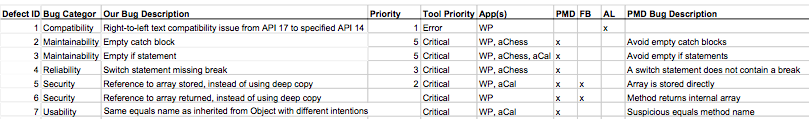
\includegraphics[width=0.45\textwidth]{images/aggregate_oracle.png}
%%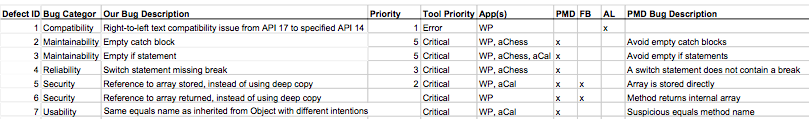
\includegraphics{images/aggregate_oracle.png}
%%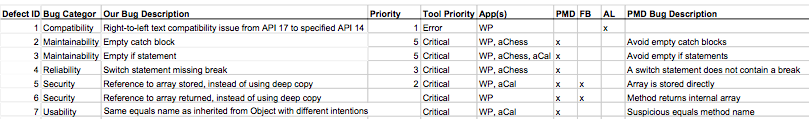
\includegraphics[width=18cm,height=5cm,keepaspectratio]{images/aggregate_oracle.png} % Backup aspect ratio
%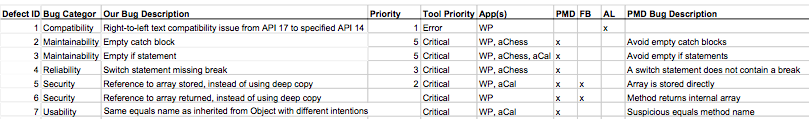
\includegraphics[width=18cm,height=3.25cm]{images/aggregate_oracle.png}
%
%\caption{Portion of Aggregate App Oracle from Website\todo{something is wrong here. Duplicate info}}
%\label{fig:aggregate_oracle}
%\end{figure*}

\begin{figure}
\centering
%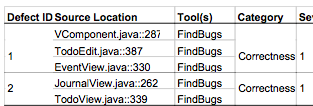
\includegraphics[width=8cm,height=2.7cm]{images/oracle_aCal1_small.png}
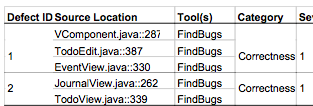
\includegraphics{images/oracle_aCal1_small.png}
\caption{Portion of aCal Oracle from Website}
\label{fig:aCalOracle}
\end{figure}





This data may be useful for future researchers in a variety of ways. The oracle may be used as a small benchmark to evaluate new tools in not only terms of precision, recall and F-measure, but also to see what categories and priority levels each tool is capable of discovering. Finally, this represents an unbiased oracle since it was not created to show the effectiveness of one tool over another. This means that other researchers should feel confident when using it to evaluate their tools.\\


\section{Limitations \& Future Work}
\label{sec:limitations}

The goal of this study is to provide the research community with an analysis of three leading static testing tools for Android applications. Our results are based on a defect oracle that was constructed by running three different tools on three different applications. The size of our oracle imposes a threat to the values of the metrics to calculate the efficiency of a tool, as a defect oracle constructed from a relatively larger pool of applications could have fine-tuned our result data set.

In this research we only took high priority bugs into consideration based on each tool's configuration. This approach was used due to the large number of defect patterns defined for each tool. In future work, considering all priority levels would give a finer result set with accurate values of precision, recall and F-measure.

%%% Makes our work look bad
%In this research we did not take into account where in the code, or application, the tool discovered a defect. It was recognized that some tools would find the same defect but in a different application. It would be beneficial to take into account where the bug was discovered and if a tool can detect it consistently in different applications. This would provide data about how accurate a tool is discovering its own defect patterns.

In the future, the defect oracle may be expanded beyond the fifty high priority defect patterns, which would allow for more fine-tuned effectiveness statistics. Once a sufficient amount of defect patterns have been prioritized and categorized in the defect oracle, the three static analysis tools should be run against a larger number of mobile applications to verify potential defects are being identified. There are always new testing tools which may be evaluated. Three other leading tools which could be analyzed are MonkeyRunner\footnote{\url{http://developer.android.com/tools/help/MonkeyRunner.html}}, Ranorex\footnote{\url{http://www.ranorex.com}}, and Appium\footnote{\url{http://appium.io}}.

%Future work should also focus on providing empirical evidence correlating a poor quality mobile application release to declining users and a high quality mobile application release to increasing users. %In the end, one could put a price tag on not only running static analysis tools, but running them in a strategic and targeted manner.


%% Move this to a different section?
Although static analysis tools have demonstrated their value on numerous occasions, it is unreasonable to expect that any tool will ever be flawless and that no static analysis tool is perfect and generally inherently contain limitations~\cite{chess2004static}. No static analysis detection tools can be expected to perfectly discover every bug in every scenario, and many limitations in FindBugs, and PMD have been noted in previous work~\cite{Thung:2012:EWD:2351676.2351685}. For example, FindBugs is only capable of discovering pre-defined bug patterns, so any defects that have not already been defined for the tool will not be reported~\cite{FindBugs_URL}. The goal of our work was to merely evaluate and compare the effectiveness of these tools, and was not to make a case either for or against using these tools in Android projects.


% Findbugs false warnings is 50% \footnote{\url{http://findbugs.sourceforge.net/factSheet.html}}

% Unreasonable to expect that our oracle of XXX issues represents all variations and types of defects.

%% Describe these tools in further detail


%% Compare with more bugs from more categories



\section{Conclusion}
\label{sec:conclusion}

The ability to effectively automatically identify potential software defects in mobile applications using static analysis tools is paramount for improving the overall quality of the app; therefore, improving the likelihood of attracting and retaining users. We analyzed three leading Android static analysis testing tools and compared them in a variety of ways using a new, and publicly accessible defect oracle. While none of the three evaluated tools led in all three categories of precision, recall and F-measure, FindBugs performed at the most consistently high level and led in the categories of Recall and F- Measure in comparison to PMD and Android Lint. PMD and FindBugs were able to discover the most bug categories. We also created a robust, and unbiased public defect oracle which we hope will be used by future researchers.


%This research provided an in depth analysis on the effectiveness of three static analysis tools at finding software defects in Android mobile applications. To perform the evaluation, a defect oracle was created, which contains a database of various types of software defects. Each tool was ran on three different Android apps: aCal, android-chess, and WordPress. All discovered defects were then mapped to the unique defect identifier in the defect oracle. Using this data we were able to calculate statistics and provide recommendations based on our initial research questions. Based upon our analysis, we found that FindBugs discovered the best collecting rating of precision, recall and F-measure.

%%% Make further mention of the research questions?


\balance
\bibliographystyle{abbrv}
\bibliography{AndroidTestingTools}

% That's all folks!
\end{document}


%%% Submission Location
%	Confirmation Number: 1032
%	Submission Passcode: 1032X-F7A6B3J3F8

% https://www.softconf.com/f/sac2016/cgi-bin/scmd.cgi?scmd=aLogin&passcode=1032X-F7A6B3J3F8





%%%
% Make sure that F-score/F-measure are consistent
% Proofread much more


% Project data
%	https://drive.google.com/drive/folders/0B-73wTwT9OkVTzRWb3hpQVlSX0U



